%%%%%%%%%%%%%%%%%%%%%%%%%%%%%%%%%%%%%%%%%%%%%%%%%%%%%%%%%%%%%%%
%
% Welcome to writeLaTeX --- just edit your LaTeX on the left,
% and we'll compile it for you on the right. If you give
% someone the link to this page, they can edit at the same
% time. See the help menu above for more info. Enjoy!
%
%%%%%%%%%%%%%%%%%%%%%%%%%%%%%%%%%%%%%%%%%%%%%%%%%%%%%%%%%%%%%%%

% --------------------------------------------------------------
% This is all preamble stuff that you don't have to worry about.
% Head down to where it says "Start here"
% --------------------------------------------------------------
 
\documentclass[12pt]{article}
 
\usepackage[margin=1in]{geometry}
\usepackage{amsmath,amsthm,amssymb}

\usepackage{listings}
\usepackage{xcolor}
\usepackage{circuitikz}
\usetikzlibrary{bending}
\usetikzlibrary{patterns,decorations.pathmorphing,positioning}
\usepackage{float,graphicx}

%New colors defined below
\definecolor{codegreen}{rgb}{0,0.6,0}
\definecolor{codegray}{rgb}{0.5,0.5,0.5}
\definecolor{codepurple}{rgb}{0.58,0,0.82}
\definecolor{backcolour}{rgb}{0.95,0.95,0.92}

%Code listing style named "mystyle"
\lstdefinestyle{mystyle}{
  backgroundcolor=\color{backcolour}, commentstyle=\color{codegreen},
  keywordstyle=\color{magenta},
  numberstyle=\tiny\color{codegray},
  stringstyle=\color{codepurple},
  basicstyle=\ttfamily\footnotesize,
  breakatwhitespace=false,         
  breaklines=true,                 
  captionpos=b,                    
  keepspaces=true,                 
  numbers=left,                    
  numbersep=5pt,                  
  showspaces=false,                
  showstringspaces=false,
  showtabs=false,                  
  tabsize=2
}

%"mystyle" code listing set
\lstset{style=mystyle}

 
\newcommand{\N}{\mathbb{N}}
\newcommand{\Z}{\mathbb{Z}}
 
\newenvironment{theorem}[2][Theorem]{\begin{trivlist}
\item[\hskip \labelsep {\bfseries #1}\hskip \labelsep {\bfseries #2.}]}{\end{trivlist}}
\newenvironment{lemma}[2][Lemma]{\begin{trivlist}
\item[\hskip \labelsep {\bfseries #1}\hskip \labelsep {\bfseries #2.}]}{\end{trivlist}}
\newenvironment{exercise}[2][Exercise]{\begin{trivlist}
\item[\hskip \labelsep {\bfseries #1}\hskip \labelsep {\bfseries #2.}]}{\end{trivlist}}
\newenvironment{problem}[2][Problem]{\begin{trivlist}
\item[\hskip \labelsep {\bfseries #1}\hskip \labelsep {\bfseries #2.}]}{\end{trivlist}}
\newenvironment{question}[2][Question]{\begin{trivlist}
\item[\hskip \labelsep {\bfseries #1}\hskip \labelsep {\bfseries #2.}]}{\end{trivlist}}
\newenvironment{corollary}[2][Corollary]{\begin{trivlist}
\item[\hskip \labelsep {\bfseries #1}\hskip \labelsep {\bfseries #2.}]}{\end{trivlist}}

\newenvironment{solution}{\begin{proof}[Solution]}{\end{proof}}
 
\begin{document}
 
% --------------------------------------------------------------
%                         Start here
% --------------------------------------------------------------
 
\title{Lab 2}%replace X with the appropriate number
\author{Mengxiang Jiang\\ %replace with your name
CSEN 5303 Cybersecurity} %if necessary, replace with your course title
 
\maketitle
 
\begin{problem}{1} %You can use theorem, exercise, problem, or question here.  Modify x.yz to be whatever number you are proving
Command Line Interface Management

\begin{enumerate}
    \item Launch the Windows command prompt. If you are not in your \verb|Users| directory (folder), change to that location.
    \begin{figure}[H]
        \centering
        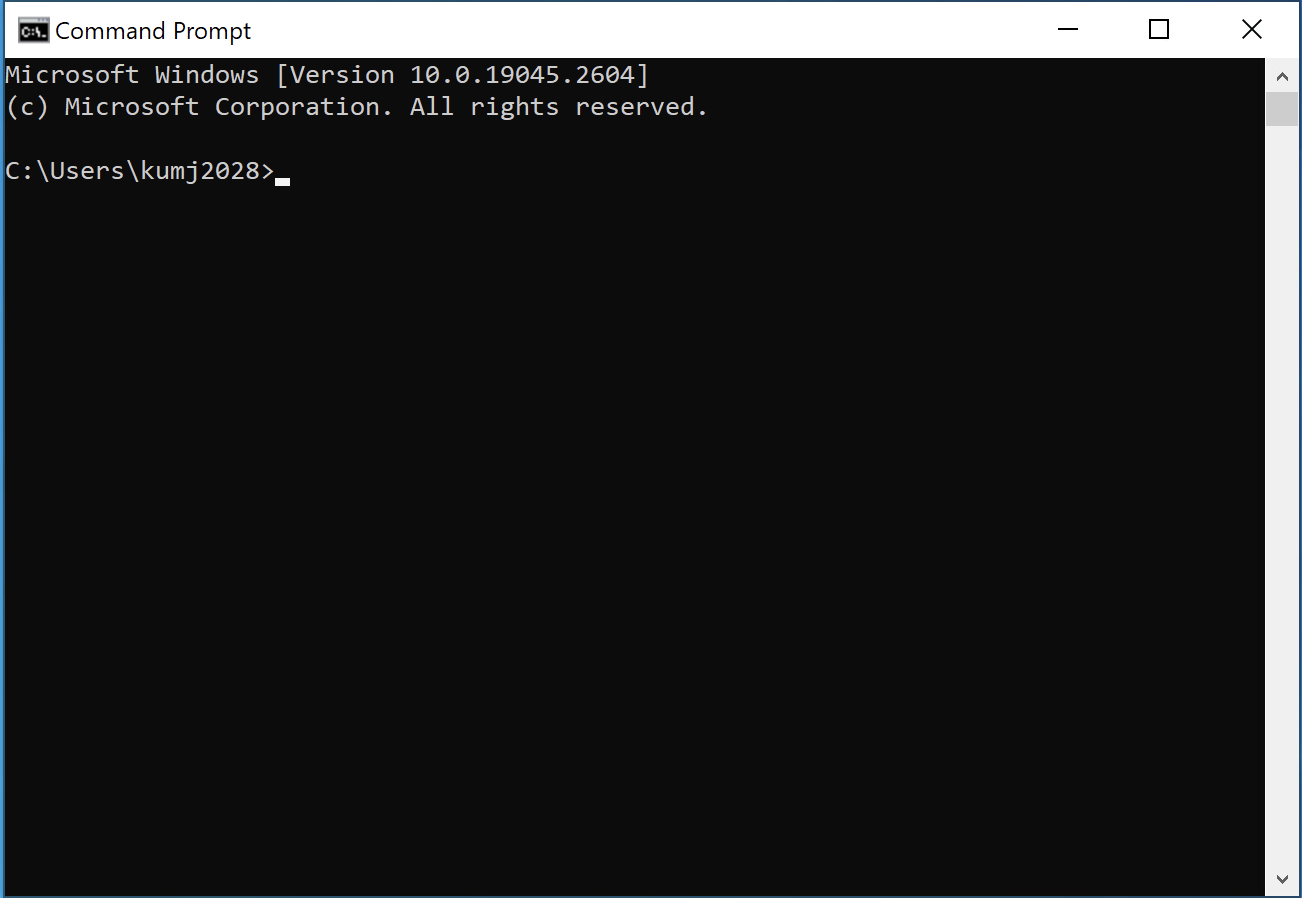
\includegraphics[width=0.7\textwidth]{cmd}
        \caption{Command Prompt Start Screen}
    \end{figure}
    \pagebreak
    \item Within your Users directory, make a new directory called \verb|MyFiles|. What do you enter to create this directory?
    \begin{verbatim}
        md MyFiles
    \end{verbatim}
    \begin{figure}[H]
        \centering
        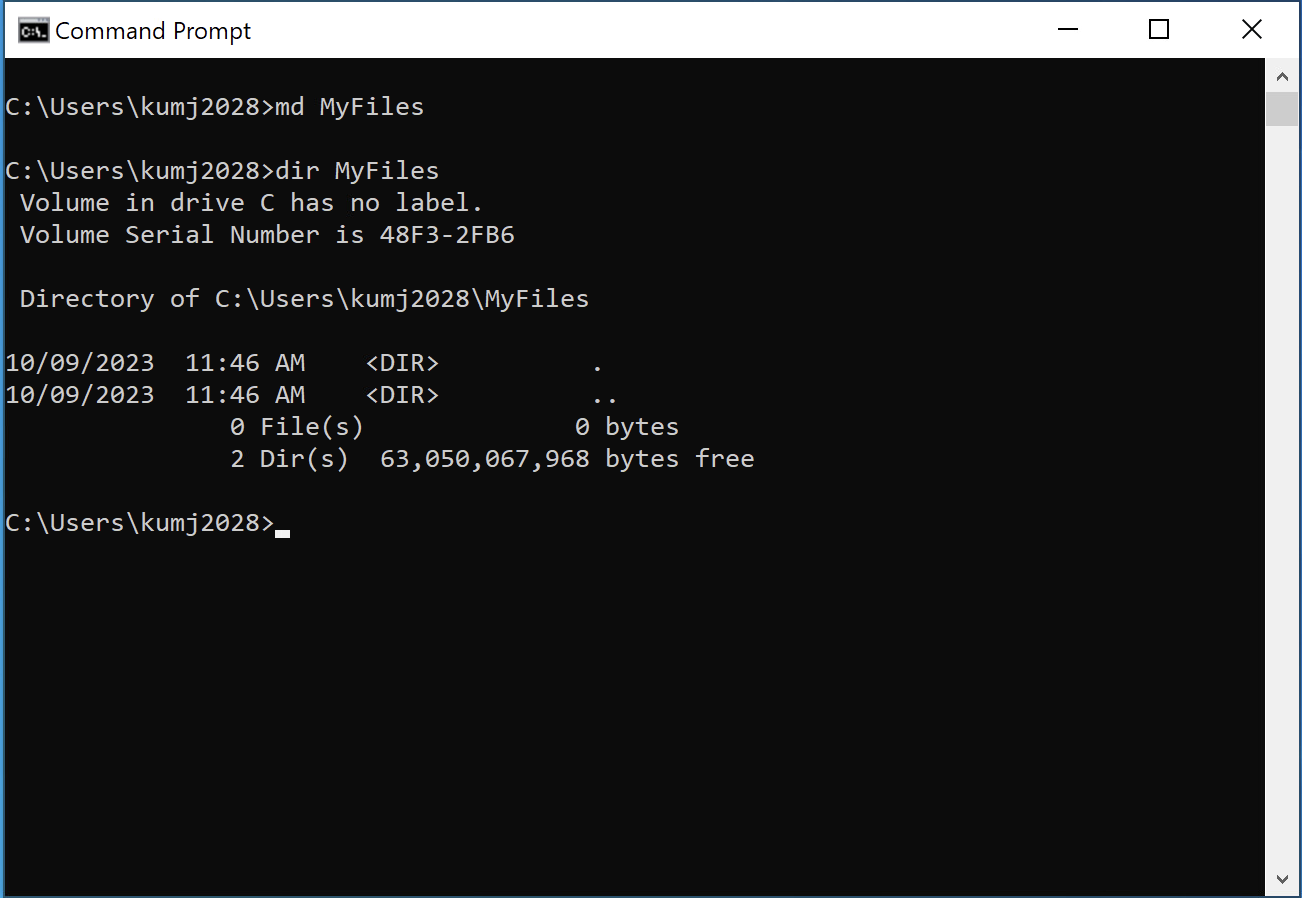
\includegraphics[width=0.7\textwidth]{md}
        \caption{Creating Directory MyFiles}
    \end{figure}
    \item Run the command \textbf{TREE} to see the subdirectories from your Users directory. Create and save a screenshot.
    \begin{figure}[H]
        \centering
        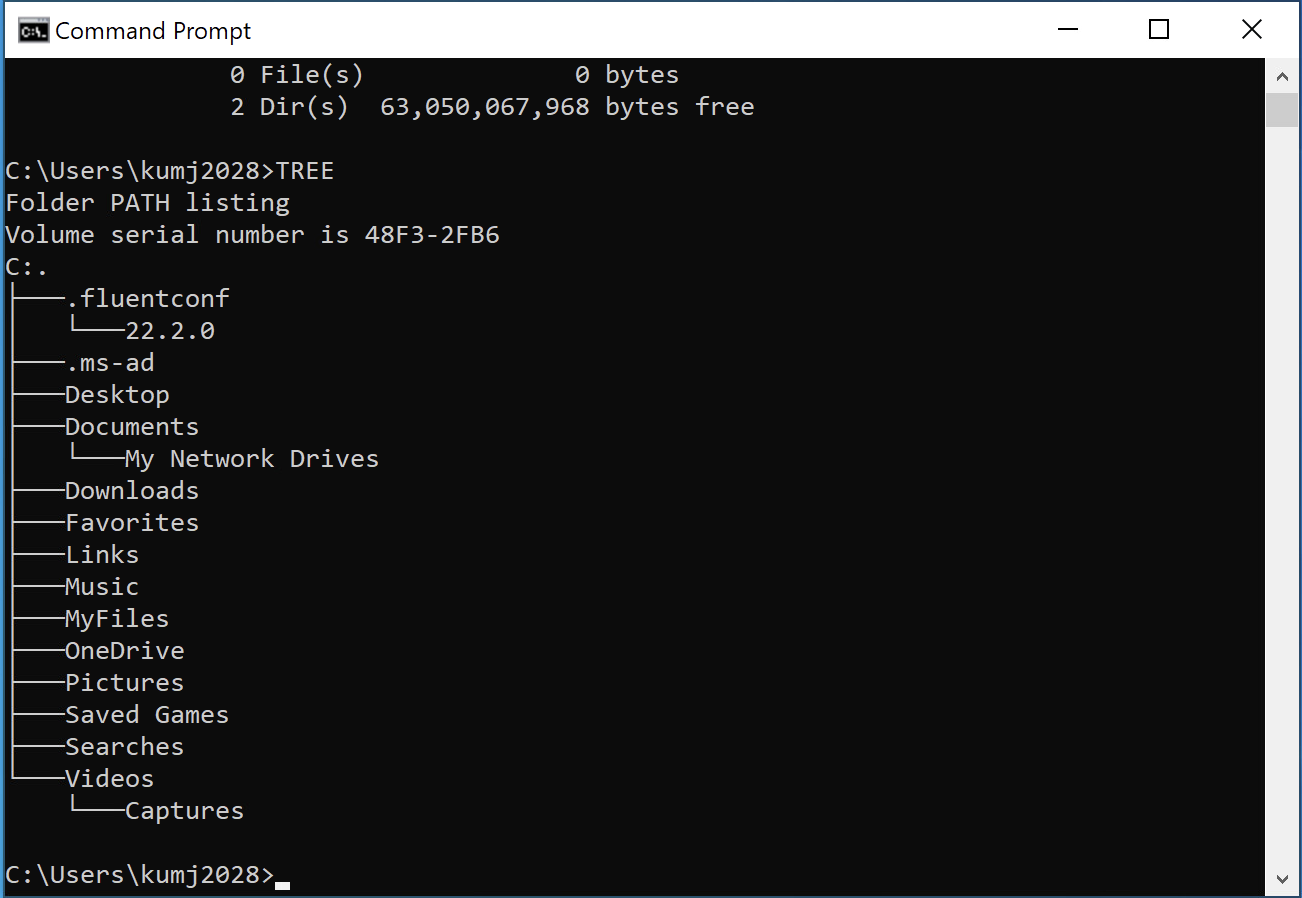
\includegraphics[width=0.7\textwidth]{tree}
        \caption{Running \textbf{TREE} on Users directory}
    \end{figure}
    \item Change to the \verb|C:\Windows| directory. Search the directory for all files starting with the letter S. What do you enter for this? Create and save a screenshot.
    \begin{verbatim}
        dir \S S*
    \end{verbatim}
    \begin{figure}[H]
        \centering
        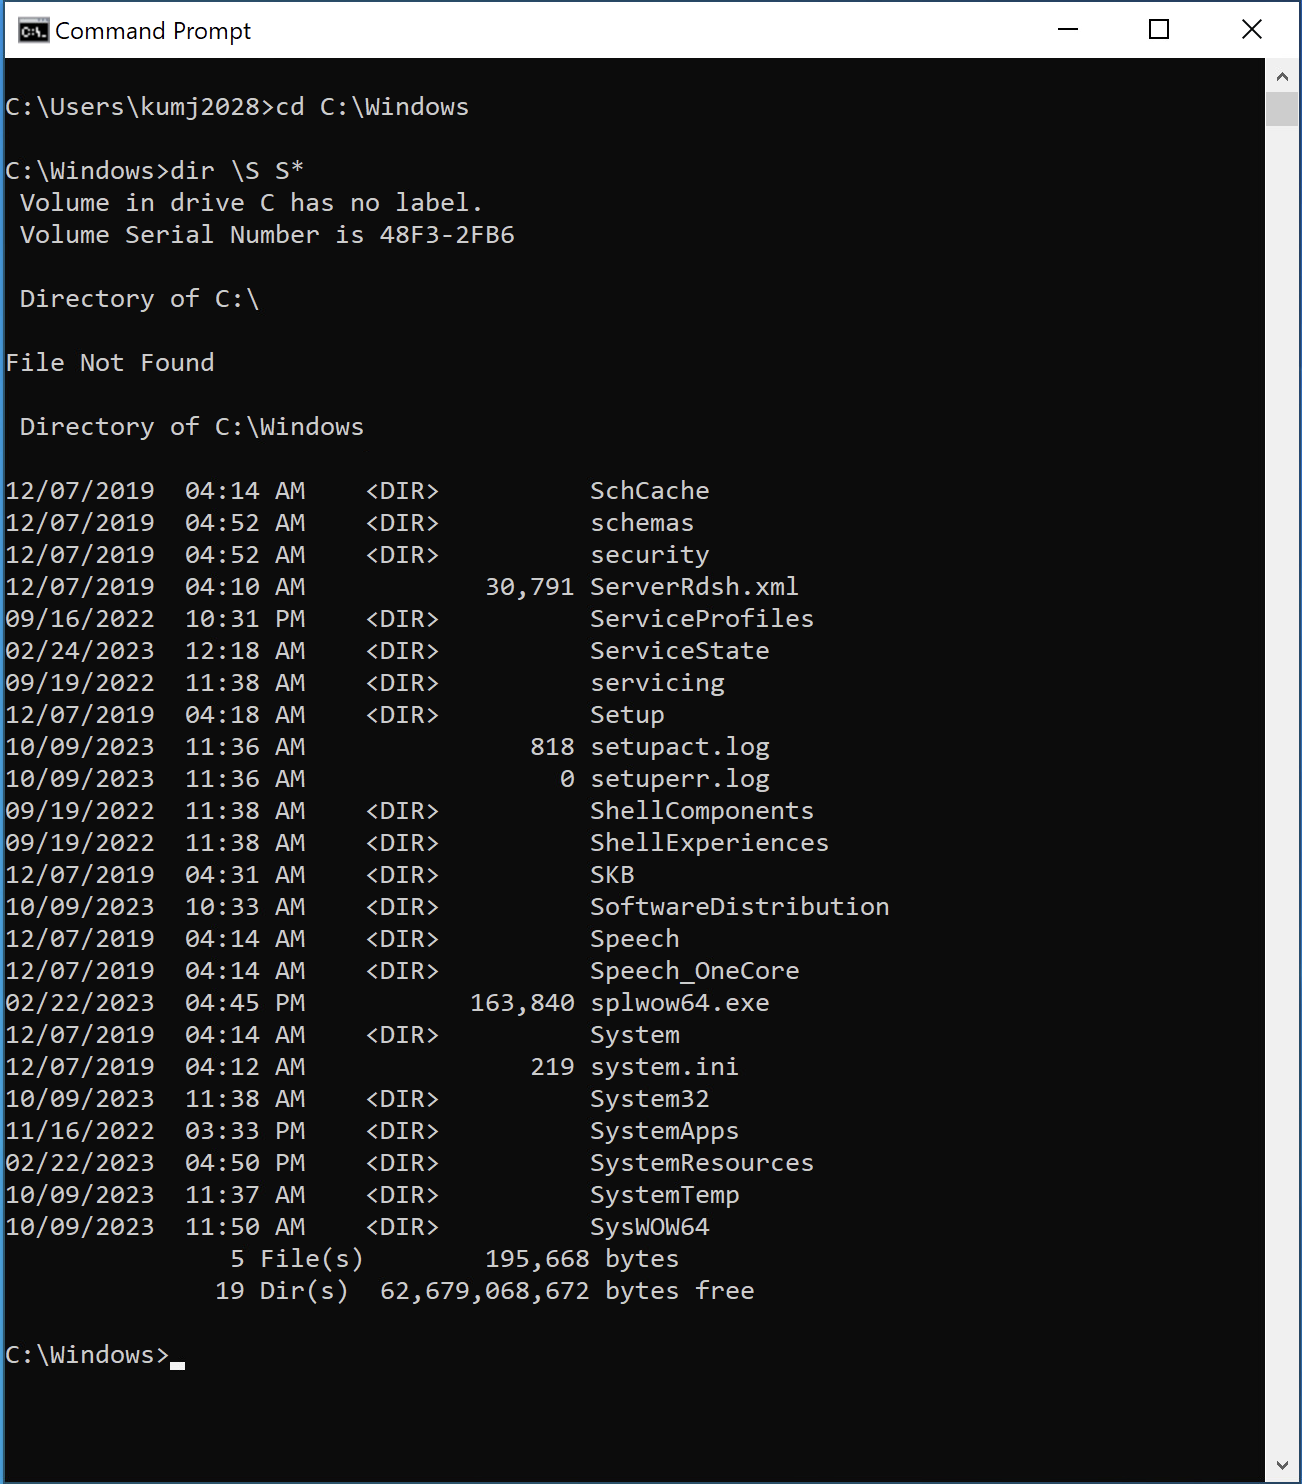
\includegraphics[width=0.7\textwidth]{dir}
        \caption{Searching for all files starting with S on the Windows directory}
    \end{figure}
    \pagebreak
    \item Show all files with a \verb|.ini| file extension. What do you enter for this? Create and save a screenshot.
    \begin{verbatim}
        dir \S *.ini
    \end{verbatim}
    \begin{figure}[H]
        \centering
        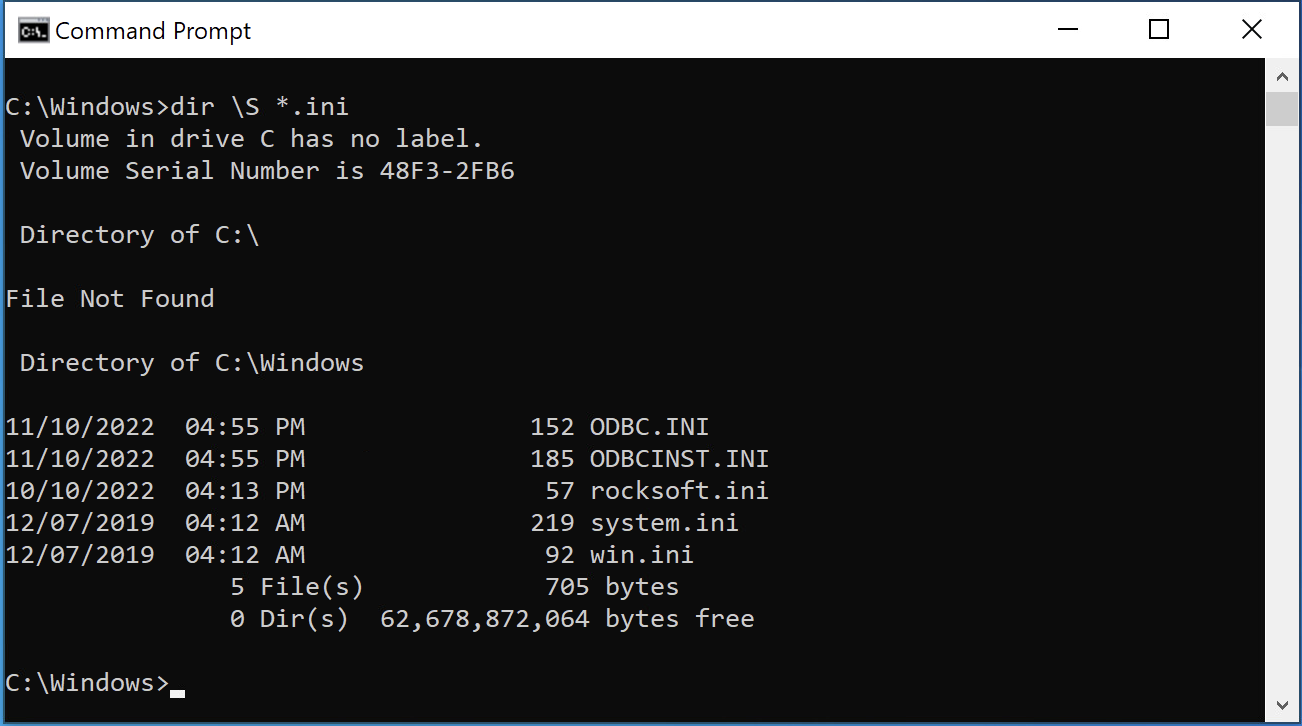
\includegraphics[width=0.7\textwidth]{ini}
        \caption{Searching for all .ini extension files on the Windows directory}
    \end{figure}
    \item Using the \verb|/?| switch, determine the command and options to show all the files in order by reverse date. Pause the screen so you can see this. What do you enter for this? Create and save a screenshot.
    \begin{verbatim}
        dir \O-D \P
    \end{verbatim}
    \begin{figure}[H]
        \centering
        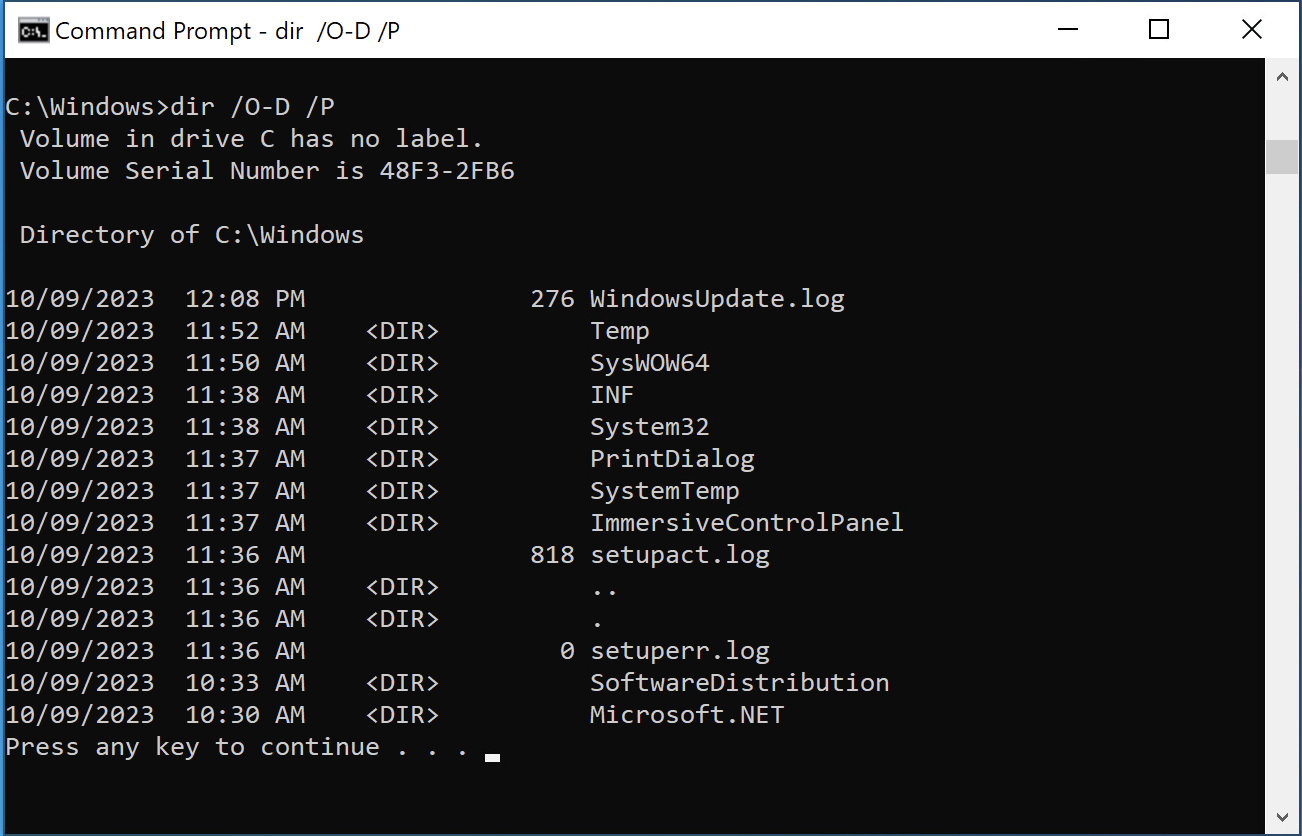
\includegraphics[width=0.7\textwidth]{sort}
        \caption{Sorting the files by the most recent first}
    \end{figure}
    \item Navigate to your \verb|Users| directory.
    \begin{figure}[H]
        \centering
        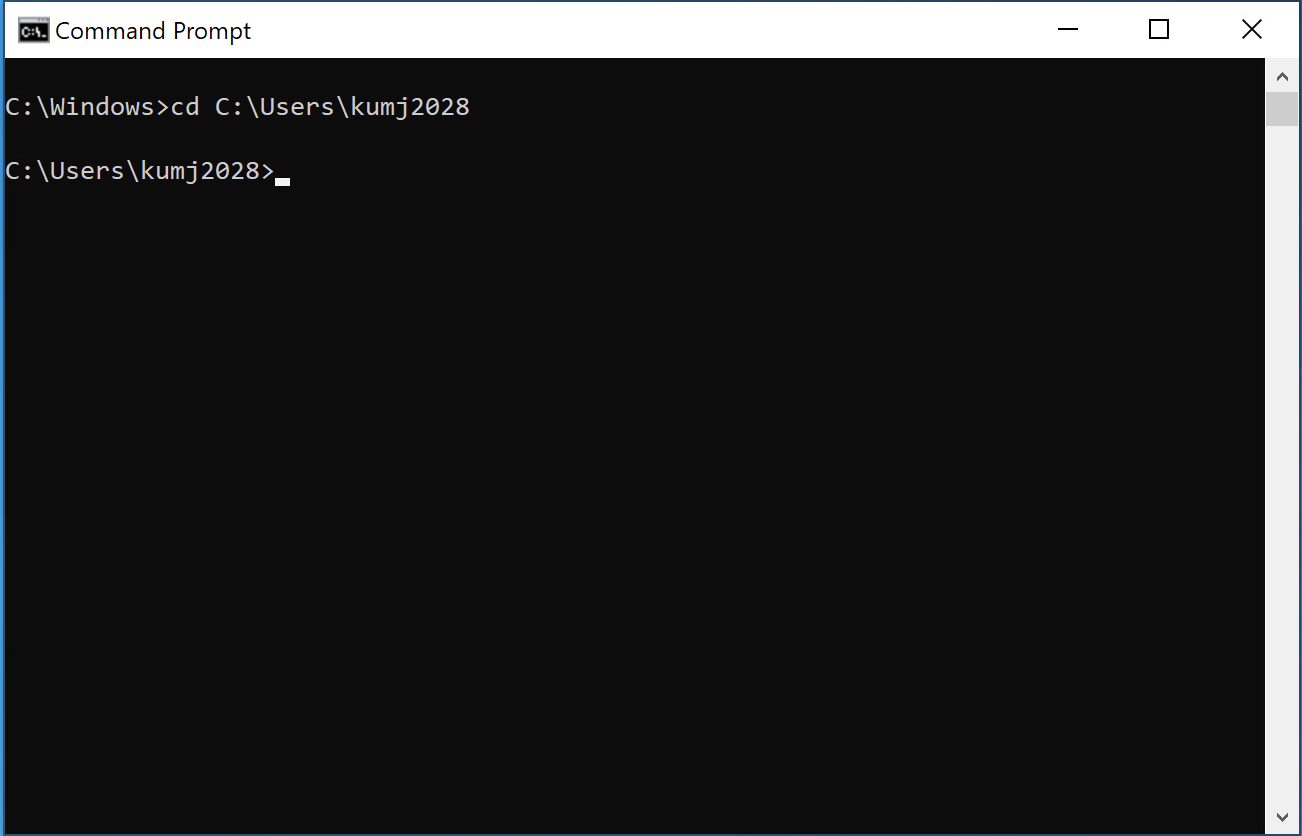
\includegraphics[width=0.7\textwidth]{cd}
        \caption{Back to Users}
    \end{figure}
    \item Run the textbf{IPCONFIG} command, and redirect the output to a file called \verb|MyIP.txt|. What do you enter for this? Create and save a screenshot.
    \begin{verbatim}
        ipconfig > MyIP.txt
    \end{verbatim}
    \begin{figure}[H]
        \centering
        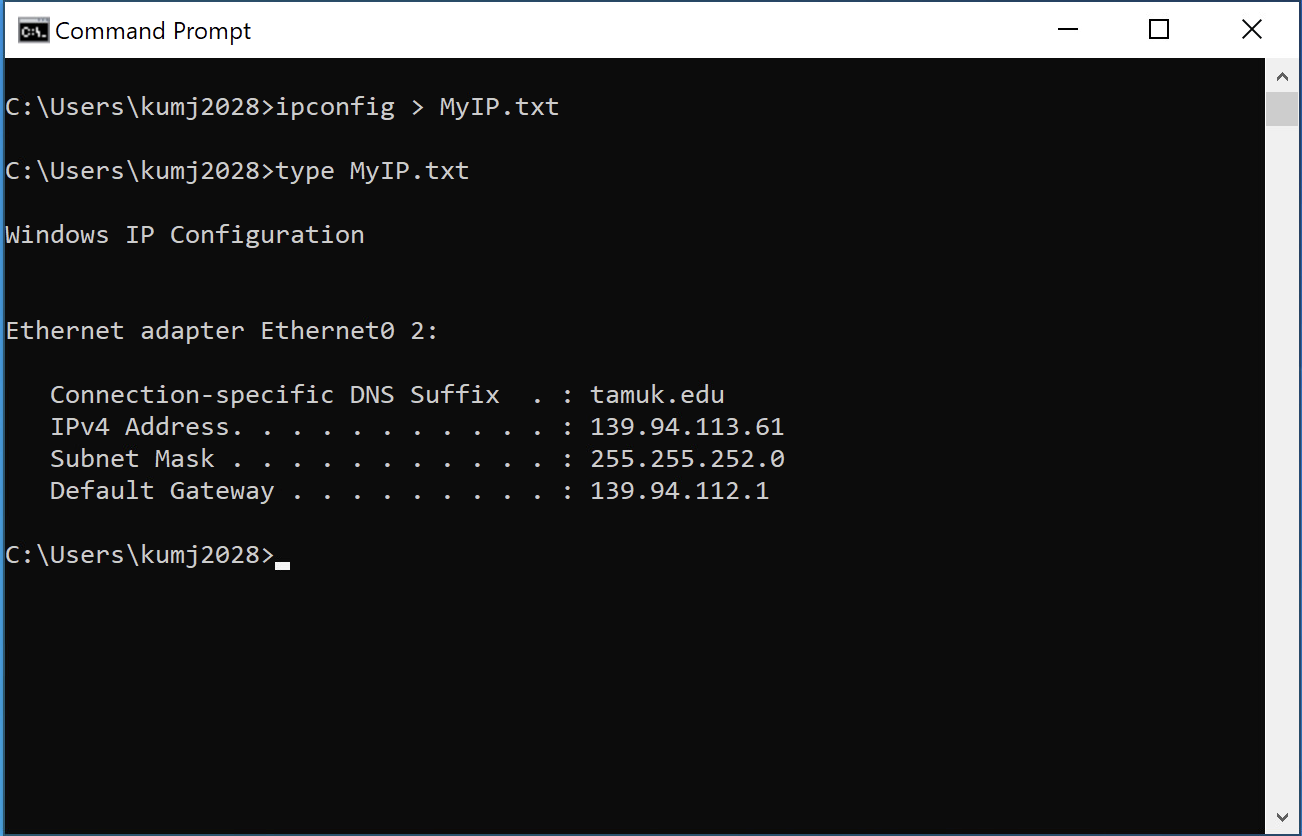
\includegraphics[width=0.7\textwidth]{ipconfig}
        \caption{Running \textbf{IPCONFIG} and redirecting the output to a file}
    \end{figure}
\end{enumerate}

\end{problem}
% --------------------------------------------------------------
%     You don't have to mess with anything below this line.
% --------------------------------------------------------------
 
\end{document}